\documentclass[12pt,twoside]{reedthesis}

% Default Thesis Packages:
\usepackage{graphicx,latexsym} 
\usepackage{amssymb,amsthm,amsmath}
\usepackage{longtable,booktabs,setspace} 
\usepackage[hyphens]{url}
\usepackage{rotating}
\usepackage{natbib}

% Added by me:
\usepackage{enumitem}
\newenvironment{halfpage}{\begin{minipage}{0.5\textwidth}}{\end{minipage}}
\usepackage{braket}
\usepackage{tristan-math}
\theoremstyle{definition}\newtheorem{definition}{Definition}
\theoremstyle{definition}\newtheorem{example}{Example}
\theoremstyle{plain}\newtheorem{postulate}{Postulate}
\theoremstyle{plain}\newtheorem{theorem}{Theorem}
\usetikzlibrary{arrows, shapes.gates.logic.US, calc}
\usepackage{qcircuit}

% Editing/Debugging
\newcommand{\TODO}[1]{{ \color{red} \textbf{TODO}: {#1}}}
\newcommand{\FIX}[1]{{ \color{blue} \textbf{FIX}: {#1}}}
\definecolor{background}{HTML}{F0DBB7}


\newcommand{\placeholderfig}{
    \begin{center}
        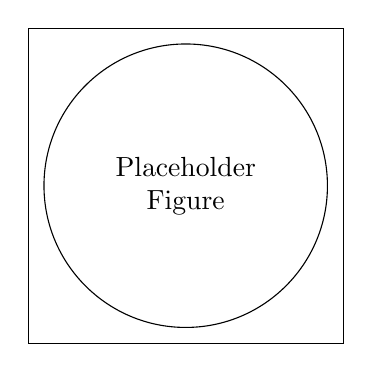
\begin{tikzpicture}
            \draw (2,2) circle (1.8cm) node[align=center] {Placeholder\\ Figure};
            \draw (0,0) rectangle (4,4);
        \end{tikzpicture}
    \end{center}
}


\includeonly{
     %content/preamble,
     %content/introduction,
     content/quantum-computing,
%     content/representation-theory,
%     content/symmetric-oracles,
%     content/results,
}

\listfiles

\begin{document}



%% Thesis information:
\title{On the Quantum Base Size of a Group}
\author{Tristan Wylde-LaRue}
% The month and year that you submit your FINAL draft TO THE LIBRARY (May or December)
\date{May 2019}
\division{Mathematics and Natural Sciences}
\advisor{Jamie Pommersheim}
%If you have two advisors for some reason, you can use the following
%\altadvisor{Your Other Advisor}
%%% Remember to use the correct department!
\department{Mathematics}






  \maketitle
  \frontmatter % this stuff will be roman-numbered
  \pagestyle{empty} % this removes page numbers from the frontmatter

% Acknowledgements (Acceptable American spelling) are optional
% So are Acknowledgments (proper English spelling)
    \chapter*{Acknowledgements}
    First and foremost, I would like to thank my family for their incredible patience and kindness, I could not 
    have made it through this without them. 

    I am extremely grateful for my advisor Jamie who guided me through all of this. It was amazing to have been 
    able to take classes with him and share in his excitement for everything math related. For thesis, he has been 
    nothing but kind and patient. Working with him has been an honor.

    Finally, I want to thank all of my friends who have put up with me this last year working on this. I have to 
    specifically thank Raina for being there for me without a second thought when I was really struggling.

% The preface is optional
% To remove it, comment it out or delete it.
    %\chapter*{Preface}
	%This is an example of a thesis setup to use the reed thesis document class.
	
	

    %\chapter*{List of Abbreviations}
		%You can always change the way your abbreviations are formatted. Play around with it yourself, use tables, or come to CUS if you'd like to change the way it looks. You can also completely remove this chapter if you have no need for a list of abbreviations. Here is an example of what this could look like:

	%\begin{table}[h]
	%\centering % You could remove this to move table to the left
	%\begin{tabular}{ll}
		%\textbf{ABC}  	&  American Broadcasting Company \\
		%\textbf{CBS}  	&  Columbia Broadcasting System\\
		%\textbf{CDC}  	&  Center for Disease Control \\
		%\textbf{CIA}  	&  Central Intelligence Agency\\
		%\textbf{CLBR} 	&  Center for Life Beyond Reed\\
		%\textbf{CUS}  	&  Computer User Services\\
		%\textbf{FBI}  	&  Federal Bureau of Investigation\\
		%\textbf{NBC}  	&  National Broadcasting Corporation\\
	%\end{tabular}
	%\end{table}
	

    \tableofcontents
% if you want a list of tables, optional
    %\listoftables
% if you want a list of figures, also optional
    %\listoffigures

% The abstract is not required if you're writing a creative thesis (but aren't they all?)
% If your abstract is longer than a page, there may be a formatting issue.
    \chapter*{Abstract}
    In this thesis we study the query complexity of quantum oracle problems in which a learner must identify a 
    hidden group element by querying its action on a set. A recent paper of Pommersheim and Copeland connects this 
    problem to a classical problem in the representation theory of finite groups. We extend their work by computing 
    the query complexity for symmetric oracle problems associated to the dihedral groups.
    
    \chapter*{Dedication}
    \emph{To my sister Cordelia who inspired my love of math}.
  \mainmatter % here the regular arabic numbering starts
  \pagestyle{fancyplain} % turns page numbering back on


\chapter*{Introduction}
\addcontentsline{toc}{chapter}{Introduction}
\chaptermark{Introduction}
\markboth{Introduction}{Introduction}


In 1994, Peter Shor showed that if a working quantum computer could be built, it would be capable of factoring 
integers exponentially faster than is thought to be possible on a classical computer. This was perhaps the most 
prominent of a series of successes that publicly established the field of quantum computing as something worth 
seriously researching. It is a very unique subject today, as it is one of the few that is truly interdisciplinary.  
Influential papers in the field are routinely published by researchers in mathematics, physics, computer science 
and even occasionally chemistry departments. 

The primary goal of this thesis is to introduce a reader familiar with linear algebra and abstract algebra to an 
interesting open problem at the intersection of quantum computing and  representation theory. The first two 
chapters seek to give a self-contained introduction to quantum computing  and representation theory respectively.  
The section on quantum computing is intended slightly towards someone with a mathematical background rather than a 
physics or computer science one. Finally, chapter three introduces the problem and the paper that motivates it and 
in chapter four explicit examples are computed.
    



\onehalfspacing

\chapter{Quantum Computing}

\section{Learning Problems}

\subsection{A Motivating Example}


        Suppose you're involved in a simple card game: A dealer places two cards\footnote{Assume that the cards are
        either red or black, with equal probability of each occurring}  face down on a table. You win the game and a
        substantial prize if you can guess whether the two face-down cards share the same color. You're allowed to
        ask the dealer to reveal cards to you, but for each card revealed your potential prize gets smaller.

        How many of the cards do you need to see to determine with certainty whether the cards share the same
        color?  Maybe you don't need to know for certain. How does the probability of you being able to guess the
        correct answer relate to the number of cards seen?


        If you have no information at all, you can't do substantially better (or worse) than a fifty-percent
        chance. In fact, seeing only a single card, does not give you any more knowledge of what the answer to the
        question is. If you wanted to know with certainty what the answer was, you would need to see both cards.


        This is of course a very simple game, but it is an example of a type of problem that we refer to as
        \emph{learning problems} or often \emph{oracle problems}. These problems consist of a learner who is trying
        to determine the answer to some question, generally to find the output of a certain function. The learner
        starts out with incomplete information, but is given access to an \emph{oracle function} she can query to
        gain more information. An oracle function--also sometimes called a black-box function--is one that you can
        evaluate the oracle at any input of your choosing, but you have no information about the function other
        than its responses to your inputs. The learner's goal is to determine the answer to the question in as few
        questions as possible. 

        We rephrase the scenario given above in this language.  Choose 0 to represent a black card and 1 to
        represent a red card. Suppose the two facedown cards are labeled $a$ and $b$.   
       
        \begin{example} 
            Given oracle access to a function $f: \{a, b\} \rightarrow \{0, 1\}$. What is the minimum number of
            queries required to determine $f(a) \oplus f(b)$ where $\oplus$ denotes addition mod 2?
        \end{example}

        
        \TODO{rewrite this example}

        Phrasing problems in terms of oracles is an extremely useful tool. It provides an approach for using 
        information theoretic arguments to provide algorithmic lower bounds. We know of very few tools to show that 
        there is no way to possible solve something quickly.

        \begin{example}
            \TODO{Example 2?} 
        \end{example}


        

\section{Classical Computing}
        \subsection{History, Bits, Information Theory}
        Before we delve into  \emph{quantum computation}, we first briefly give an overview of the relevant 
        concepts from the study of \emph{classical} computation. Although we will not need information theory for 
        any of the arguments we will make, it will be used frequently as a source of intuition.

        The fundamental idea of information theory is that any the amount of information that an object contains is 
        determined exactly by the number of possible states it could have been in. In this way, the bit, which can 
        be in exactly one of two possible states is the most basic unit of information.


        In the 16th and 18th centuries mathematicians and logicians worked to convert formal systems of logic into 
        algebra and arithmetic. One of the most prominent successes of these attempts was by George Boole who 
        managed to faithfully encode propositional logic in the language of arithmetic and algebra. The idea was to 
        let 1 and 0 represent true and false respectively. Then, by interpreting addition and multiplication as mod 
        2, one obtains exactly the logical operations \texttt{AND} and  \texttt{XOR}. In modern terms, we recognize 
        this as the structure of the field $\F_2$. \TODO{remove this paragraph}
        
        \TODO{\textit{These next two paragraphs just repeat the previous two paragraphs, clean this up}}

        We define a bit as an element of $\Z/2\Z = \{0,1\}$. It also can be useful to think of bits as representing 
        a true or false value. This relationship gives a direct correspondence between classical computation and 
        propositional logic. We write the state space of a bit as $\Z/2\Z$ to emphasize that it has a natural 
        additive operation given by mod 2 addition.  Alluding to propositional logic, this operation is called 
        exclusive-or, usually written as \texttt{XOR} or $\oplus$, although we will oftentimes just write $+$.

        Of course having just one bit, is not particularly interesting. As a reference, it is common today to 
        measure memory in terms of \emph{gigabytes}. One gigabyte is equivalent to eight billion bits. We most 
        often work with \emph{strings of bits}. A string of 2 bits has four possible states, each described by an 
        element of $\Z/2\Z \times \Z/2\Z$. Analogously, an $n$ bit string has state space $(\Z/2\Z)^n$. The group 
        addition readily extends to $n$ bit strings giving it the operation that is commonly known as bitwise XOR.


        Thus any function $f :  \{0, 1\}^m \rightarrow \{0, 1\}^n$ can be expressed by some sequence of logical 
        operations and each sequence of logical operations corresponds to a function. 
        
        \subsection{Circuits and Logic Gates}

        \begin{definition}
            [Nielsen and Chuang, pg 129]
            A \emph{circuit} is made up of wires and gates, which carry information around, and perform simple 
            computational tasks, respectively.
        \end{definition}

        \begin{definition}
            [Nielsen and Chuang, pg 129]
            A \emph{logic gate} is a function $f : \{0, 1\}^k \rightarrow \{0, 1\}^\ell$ from some fixed number $k$ 
            of input bits to some fixed number $\ell$ of output bits.
        \end{definition}

        \begin{example}
         Here is an example of a logic gate

         \begin{figure}[ht]
            \centering
            \placeholderfig
            \caption{ The logic gates \texttt{AND} and \texttt{XOR} }
        \end{figure}
        \end{example}

        \bigskip

        \begin{example}
            Here is an example of a circuit

            \begin{figure}[ht]
                \centering
                    \placeholderfig
                \caption{An example of a basic circuit, maybe make it match whatever example I use for a circuit 
                family}
            \end{figure}

    
        \end{example}

        We state the following important result without proof.
        \begin{theorem}
            The set of gates $\{ \texttt{AND},\ \texttt{NOT},\ \texttt{OR} \}$ are \emph{universal}. That is any 
            function $f : \{0, 1\}^n \rightarrow \{0, 1\}$ can be represented by circuit a consisting of only 
            \texttt{AND}, \texttt{NOT}, and \texttt{OR} gates.
        \end{theorem}
        
        %{\textcolor{red}{\bfseries I don't know how to fill the rest of this circuit part in}}
        

        \subsection{Circuits as Algorithms}
        
        \begin{definition}
            [verbatim from Sipser -- cleanup]
                 A \emph{circuit family} is an infinite list of circuits $(C_0, C_1, C_2, ...)$, where $C_n$ has 
                 $n$ input bits.
        \end{definition}

        \begin{definition}
            The circuit complexity of a function is the size complexity of a minimal circuit family for that 
            language. 
        \end{definition}

        \begin{example}
            Example circuit family to compute something. Maybe how many input bits are odd.  
            \begin{figure}[ht]
                \centering
                    \placeholderfig
                \caption{}
            \end{figure}
        \end{example}
        
        \subsection{Introduce controlled gate notation}
        
        Just example of Toffoli gate or whatever

        \subsection{Circuits with Oracles}

        We can consider circuits with oracle access.  Give example from original motivating problem.



\section{Quantum Computing}
        Now we introduce the concepts required for quantum computation. In the quantum world, the \emph{qubit} is 
        the fundamental unit of information. In the same way that we could express any classical algorithm as a 
        circuit of logical operations on bits, we can express any quantum operation as a sequence of \emph{unitary} 
        operations on \emph{qubits}.
       
   \subsection{Qubits}

        The following definitions will give a complete description of a model of quantum computing. These can all 
        be derived from the postulates of quantum mechanics.
        
        Whereas the state of a bit has \emph{two} possible values---either 0 or 1---the state of a qubit is a unit
        vector in complex vector space spanned by \emph{two} basis states. We give the following precise definition

        Whereas a bit has two states---0 or 1---a qubit has \emph{two basis states}. The following definition makes 
        this precise
        \begin{definition}
            The state of a \emph{qubit} is a unit vector in $\C^2$. That is, a pair of complex numbers
            \[
                (\alpha, \beta) \in \C^2
            \]
            satisfying the normalization condition %
            \[
                |\alpha|^2 + |\beta|^2 = 1
            \]
        \end{definition}
        
        We refer to the space $\C^2$ as the \emph{state space} of a qubit and consider it to be an inner product 
        space equipped with the standard inner product on $\C^n$.\footnote{In quantum mechanics literature, state 
            spaces of quantum systems are always referred to as \emph{Hilbert spaces} regardless of their 
            dimension. This can be confusing as \emph{Hilbert spaces} in mathematics are generally associated with 
        infinite dimensional spaces. Since all of the spaces in this thesis will be finite dimensional (and 
    isomorphic to $\C^{2^n}$), it is easier to avoid the confusion and use the term state space instead.}
    We choose the standard basis $\{(0,1), (1,0)\}$ to represent $\C$. In order to make the analogy with bits more 
    clear, we denote \[
            \ket{0} := \rvec{1}{0}, \quad
            \ket{1} := \rvec{0}{1}.
         \] The symbol $\ket{\ }$ is called a ket and is used to denote a vector representing a quantum state. It 
         comes from the \emph{bra-ket} notation which is widely used in the greater theory of quantum mechanics.
        
        
         \subsection{Measurement} 
         
         Although a qubit has a quantum state in $\C^2$, the we cannot directly observe this quantum state. Despite 
         having what seems like a much richer state, when we try to measure qubits using any sort of detector, they 
         snap into the states $\ket{0}$ or $\ket{1}$. This of course defies any reasonable expectations one would 
         have about the world, and has raised much philosophical debate about how it should be interpreted. 
         However, regardless of what interpretation we take, it remains an experimental fact. The following 
         postulate formalizes this concept as a process called \emph{measurement in the computational basis} .

         \begin{postulate}
             Given a qubit $\psi$, we may perform \emph{measurement} of $\psi$ in the \emph{computational basis}. 
             If $\psi$ was in state $\alpha \ket{0} + \beta \ket{1}$ prior to the measurement, after the 
             measurement it will be in state $\ket{0}$ with probability $|\alpha|^2$ and $ \ket{1}$ with 
             probability $|\beta|^2.$
     \end{postulate}

        This is only a specific case of a much more general postulate of measurement in quantum mechanics. However, 
        this conception of measurement will be sufficient enough for many of the results in quantum computing and 
        all of the results that we will need to consider. A more in depth discussion of the postulates of quantum 
        mechanics and how they relate to quantum computing can be found in \cite{Nielsen&Chuang}.
        
        If we naively think of the state of a qubit as being in $\R^2$ rather than $\C^2$ by just ignoring the 
        imaginary part, we can generate some limited geometric intuition about what is going on.


        \begin{figure}[ht]
            \centering
            \begin{center}
            \begin{tikzpicture}
                 \draw[->] (0,0) -- (0,4) node[above]{$\ket{1}$};
                 \draw[->] (0,0) -- (4,0) node[right]{$\ket{0}$};
                 \draw[->, thick] (0,0) -- (2, 3.4) node[right]{$\frac{\sqrt{3}}{2}\ket{1} + \frac{1}{2}\ket{0}$};
            \end{tikzpicture}
            \end{center}
            \caption{A qubit with state $\frac{\sqrt{3}}{2}\ket{1} + \frac{1}{2}\ket{0}$ pictured in the plane by 
            ignoring the imaginary part. }
    \end{figure}

    A measurement on the pictured qubit will return 0 with probability $3/4$ and $1$ with probability $1/4$. This 
    perspective hopefully makes it clear why the state of a qubit had to be a unit vector. When written in the 
    standard basis, the coefficients of $\ket{0}$ and $\ket{1}$ correspond to the probability of a measurement 
    producing that outcome. Thus requiring that this state be a unit vector is equivalent to requiring that the 
    total probabilities sum to one.


    This also motivates the other postulate of quantum mechanics that we will need to formalize this model of 
    quantum computation. 

    \begin{postulate}
        The possible operations on quantum states are those given by \emph{unitary transformations}.
    \end{postulate}

    The unitary transformations on $\C^n$ are exactly the \emph{isometries} of $\C^n$, that is, the ones that 
    preserve the inner-product. This is, perhaps not too surprising, given that preserving the metric is necessary 
    condition to ensure that the probabilities sum to one. 

    \begin{definition}
        The set of unitary transformations on $\C^n$ can be represented as the set of $n \times n$ matrices $U$ 
        satisfying the identity $U^{-1} = U^\dagger$ where $U^\dagger$ denotes the conjugate-transpose of $U$.
    \end{definition}

    A consequence of this postulate of quantum mechanics is that quantum information cannot be destroyed without a 
    making a measurement.

    
    
\subsection{Gates}
        
        By postulate 2, the valid operations on a qubit are the $2 \times 2$ unitary matrices.
        

        This part of quantum computing can be confusing at first, since the notation constantly switches between 
        kets and matrices.

        \begin{example}
            The quantum \texttt{NOT} gate is the single qubit gate defined by
            \begin{align*}
                \ket{0} &\mapsto \ket{1} \\
                \ket{1} &\mapsto \ket{0}
            \end{align*}
            It should be noted that it is common to refer to the quantum \texttt{NOT} gate by the letter $X$.

            In standard vector notation this is
            \begin{align*}
                \rvec{1}{0} &\mapsto \rvec{0}{1} \\
                \rvec{0}{1} &\mapsto \rvec{1}{0} 
            \end{align*}

            Which gives us that the quantum \texttt{NOT} gate is represented by the matrix
            \[
                X := \rmat{0}{1}{1}{0}
            \]
        \end{example}

        
        \begin{example}
            A very important single qubit gate is the \emph{Hadamard} gate. The Hadamard gate, denoted $H$, can be 
            defined in terms of its action on the standard basis as
            \begin{align*}
                \ket{0} &\mapsto \frac{1}{\sqrt{2}}\left(\ket{0} + \ket{1}\right) \\
                \ket{1} &\mapsto \frac{1}{\sqrt{2}}\left(\ket{0} - \ket{1}\right)
            \end{align*}
            These states appear frequently and so it is common to give them their own notation.
            We define
            \[
                \ket{+} := \frac{1}{\sqrt{2}}\left(\ket{0} + \ket{1}\right)
            \]
            and
            \[
                \ket{-} := \frac{1}{\sqrt{2}}\left(\ket{0} - \ket{1}\right)
            \]

            The Hadamard gate has matrix representation
            \[
                H := \frac{1}{\sqrt{2}} \rmat{1}{1}{1}{-1}
            \]
        \end{example}

        
\subsection{Quantum Circuits}
        
        Much like in classical computation, it is convenient to represent manipulations of qubits as circuits.
        A \emph{quantum circuit} is made up of qubits, wires, and gates. It is perhaps easiest to define by giving 
        examples. 

        Consider the following very simple circuit
        \[\Qcircuit @C=1.5em @R=.7em {
                \lstick{\ket{0}} & \qw & \gate{X} & \gate{H} & \qw & \qw & \ket{-}
        }\]

        This circuit depicts a single qubit starting in state $\ket{0}$. As it travels through the wire left to 
        right, $X$ takes it to $\ket{1}$ and then $H$ takes $\ket{1}$ to $\ket{-}$. This circuit represents the 
        equation
        \[
            \ket{-} =  HX \ket{0}       
        \]
        Of course by associativity, we could have used a single gate $HX$.
        
        We allow for one special gate that is not unitary to denote measurement. The measurement gate is depicted 
        \[
            \Qcircuit @C=1em @R=.7em {
               & \qw & \meter & \cw 
       }\]
        The two parallel lines indicate that the wire is carrying classical information.


\subsection{Multiple qubits} 

        Up until this point we have only considered single-qubit systems. However, computation is not very 
        interesting if we're only restricted to a single qubit. 

        Consider a string of two bits. This string has four possible values: 00, 01, 10, 11. Much like in the 
        single bit case, while a string of two bits has four possible states, a string of two qubits has four basis 
        states. Keeping with the analogy from before, we number these basis vectors in binary and call them $ 
        \ket{00}, \ket{01}, \ket{10}, \ket{11}$ which represent $(1,0,0,0), (0,1,0,0), (0,0,1,0),$ and $(0,0,0,1)$ 
        respectively.

        Formally, we think of the state space of a pair of qubits as being $\C^2 \otimes \C^2$, where $\otimes$ 
        denotes the tensor product of two vector spaces. The tensor product is a complicated construction and 
        defining it in full generality here would take us beyond the scope of this thesis. Luckily, all of the 
        spaces we are working with are finite and we have already chosen bases, so we don't need to worry about 
        this. For the purposes of quantum computing the following definition is sufficient.

        \begin{definition}
            Let $V$ and $W$ be vector spaces with bases $\{v_1,...v_n\}$ and $\{w_1, ...w_m\}$ respectively.
            Define $B$ to be the set of all formal pairs $v_i \otimes w_j$. 

            The tensor product $V \otimes W$ is given by $\span B$.
        \end{definition}

        In general the state space of an $n$-qubit system is $\C^{\otimes 2n}$.


        
 
We can have circuits with multiple qubits

        \[\Qcircuit @C=1em @R=.7em {
                \lstick{\ket{0}} & \qw & \gate{H} & \qw & \qw & \ket{+}\\
        \lstick{\ket{0}} & \gate{Z} & \gate{H} & \qw & \qw & \ket{-}
        }\]
        
        

        Let \begin{example}
            Deutsch-Josza
            $$
            \Qcircuit @C=1em @R=.7em {
                & \gate{H} & \gate{Z} & \gate{H} & \qw \\
                & \qw & \gate{X} & \qw & \qw
            }
            $$
        \end{example}

        The Deutsch-Josza Algorithm 
    
            \subsection{The Bernstein-Vazirani Algorithm}
            
            \begin{problem}
                Let $s \in \{0, 1\}^m$ be a hidden $m$-bit binary string and let $b \in \{0, 1\}$ be a hidden bit.  
                Given oracle access to a function $f : \{0, 1\}^n \rightarrow \{0, 1\}$ defined by
                $f(\vec{x}) = \vec{x} \cdot \vec{s} + b \ (\text{mod } 2)$, how many queries are required to determine 
                the values of $\vec{s}$ and $b$?
            \end{problem}

            \textbf{The Bernstein Vazirani Algorithm}

            
            Define a circuit with state space $\C^{\otimes 2n} \otimes \C^2$. We initialize the system by setting 
            the first $n$ qubits to $\ket{1}$ and the response qubit to $\ket{0}$.

            The key to this problem will be to utilize a technique sometimes known as the \emph{phase-kickback 
            trick}. 
            
            
            \[
                \Qcircuit @C=1em @R=1em {
               \lstick{\ket{1}} & \qw &
               \qw \ar@{.}[]+<-0em,1em>;[d]+<-0em,-6.3em>&
                     \gate{H} & \qw &
                     \qw \ar@{.}[]+<-0em,1em>;[d]+<-0em,-6.5em>&
                    \ctrl{1} & \qw &
                    \qw \ar@{.}[]+<-0em,1em>;[d]+<-0em,-6em>&
                    \gate{H} & \qw &
                    \meter 
                    \\
                \lstick{\ket{1}} & \qw &\qw &
                    \gate{H} & \qw &\qw &
                    \ctrl{1} & \qw &\qw &
                    \gate{H} & \qw &
                    \meter 
                      \\
                \lstick{\ket{1}} & \qw &\qw &
                    \gate{H} & \qw &\qw &
                    \ctrl{1} & \qw &\qw &
                    \gate{H} & \qw &
                    \meter 
                      \\
                 \frac{1}{\sqrt{2}} &  \qw &\qw &
                     \qw &\qw &
                     \qw &                
                     \gate{U} & \qw &
                     \qw &  \qw &
                     \qw \frac{1}{\sqrt{2}} \\
               && 0 &  &  & 1 &  &  &2  & &
            }
           \]
           


        


\chapter{Representation Theory of Finite Groups}

\section{Introduction}


%Representation theory is a very powerful tool for analyzing groups. Representation theoretic tools give much more 
%profound insight into much of group theory that can be hard to find without it. The idea of representation theory, 
%is to study groups by looking at how they act on vector spaces. This allows us to use the tools of linear algebra 
%to study groups. In particular, under the right conditions, we will see that quantum oracles naturally give us 
%unitary representations of their underlying groups.

The purpose of this chapter will be to introduce the terminology and results from representation theory that we 
will need to investigate symmetric oracle problems in chapters 3 and 4. A reader familiar with the basic results of 
the representation theory of finite groups can skip ahead to chapter 3. 

This treatment of representation theory largely follows \cite{James&Liebeck}. I have omitted many proofs here and 
instead leave the reader to refer to \cite{James&Liebeck}

\section{Representations}

In this thesis, we will assume that all representations are over $\C $ if not explicitly stated.

\begin{definition}
    A \emph{representation} of a group $G$ over $\C$ is a homomorphism $\rho$ from $G$ to $\GL(n,F)$, for some $n$. 
    The degree of $\rho$ is the integer $n$.

    We say that $\rho$ is a \emph{faithful} representation if $G \cong \rho(G)$.
\end{definition}

\begin{definition}
    Let $G$ be a group and $V$ be a vector space over a field $F$. A \emph{representation} of $G$ is a homomorphism 
    $\rho : G \rightarrow \Aut(V)$, where $\Aut(V)$ denotes the group of linear maps from $V$ to itself. Although, 
    the representation is defined by the homomorphism $\rho$, it is common instead to refer to it by the space its 
    acting on.

    Equivalently, a representation can be characterized as an action of a group $G$ on a vector space $V$. In this 
    case, the action is required to be compatible with the vector space structure on $V$. That is, in addition to 
    the requirements for an action of a group on a set, we must have
\[g \cdot (\alpha v_1 + v_2) = g\cdot \alpha(v_1) + g\cdot(v_2)\]
    for all $g \in G,\ v_1, v_2 \in V,$ and $\alpha \in F$.
    We denote the action of $g \in G$ on a vector $v$ as $g \cdot v$ or $gv$.
\end{definition}

For this thesis, we will only need to consider representations of finite groups over $\C$.

We say a representation $\rho$ is \emph{faithful} if $G \cong \rho(G)$.

The degree of a representation is the dimension of $V$.

 
\begin{definition}
    Let $\rho$ be a representation of a group $G$ on a vector space $V$. A \emph{subrepresentation} is a vector 
    subspace $W \subset V$ that is invariant under the action of $G$.\footnotemark That is, for all $g\cdot w \in 
    W$ for all $g \in G$, $v \in W$.
    
    An representation is said to be irreducible if it has no nontrivial subrepresentations (the only $G$-invariant 
    subspaces of $V$ are $\{ 0 \}$ and $V$ itself).
\end{definition}


\begin{theorem}[Maschke's Theorem]
    Let $G$ be a finite group and $V$ a representation of $G$ over $\C$. If $W$ is a subrepresentation of $V$, then 
there is a subrepresentation $W'$ such that $V = W \oplus W'$.  
\end{theorem}




\begin{proof}
    Define $\pi : V \rightarrow W$ to be the projection of $V$ onto $W$. TODO rest of proof

\end{proof}


\begin{theorem}[Schur's Lemma]
    If M and N are two finite-dimensional irreducible representations of a group $G$, and $\varphi:M->N$ is a 
    linear transformation that commutes with the action of the group, then $\varphi$ is either an isomorphism or 
    the $0$ map.
\end{theorem}

%\begin{theorem}[Schur's Lemma]
    %Let $V$ and $W$ be irreducible \CG-modules.

    %\begin{enumerate}
        %\item If $\varphi : V \rightarrow W$ is a \CG-homomorphism, then either $\varphi$ is a \CG-isomorphism, or 
            %$v\varphi = 0$ for all $v \in V$. 
            
        %\item If $\varphi V \rightarrow V$ is a \CG-isomorphism, then $\varphi$ is a scalar multiple of the 
            %identity endomorphism $1_v$.
    %\end{enumerate}
%\end{theorem}

\begin{proof}
    I'll almost certainly include this one.
\end{proof}


\section{Character Theory}

One of the most surprising tools in representation theory is \emph{characters}. It's a pain to have to associate an 
entire matrix to each element of our group. What would happen if we just wrote down the trace of each matrix 
instead?



%Recall from linear algebra that the trace can be equivalently defined as the sum of the eigenvalues of a matrix. 
%This result makes it clear that the trace, and thus characters, are invariant under change of basis. This is the 
%key part of the remarkable properties that the trace seems to have, one might think of it as, the simplest 
%invariant of linear maps (depending on how simple you find its cousin, the determinant to be).


%Much in the same way that we think of the relationship between matrices and linear maps to be defined `up to change 
%of basis', we might think that groups themselves are also only defined up to inner automorphism.

%Although character theory is just a shadow of the representation theory above it, the characters of a group carry a 
%surprising amount of information about it. In fact, understanding the character theory of a group, is one of the 
%best ways to study the representation theory of a group.

%All of this prose was just written in like 30 seconds. I have no actual idea if any of this is readable or at all 
%true. Anyways, back to the math.

\begin{definition}
    Let $\rho : G \rightarrow V$ be a representation. The map $\chi : G \rightarrow \C$ given by $\chi(g) = 
    \text{Tr}\,\rho(g)$ is called the \emph{character} of $V$.
\end{definition}

\begin{definition}
    Let $G$ be a group. We say that $\chi$ is a character of $G$ if it is the character of some representation of 
    $G$.

    Moreover, if $\chi$ is the character of an irreducible representation of $G$, we say that $\chi$ is an
    \emph{irreducible character of} $G$.
\end{definition}



We give a few basic properties of characters.
\begin{theorem}
    Let $\chi$ be a character of a group $G$. Suppose $g \in G$ and $g$ has order $m$. Then
    \begin{enumerate}
        \item $\chi(1) = \dim V$.
        \item $\chi(g)$ is a sum of $m$th roots of unity.
        \item $\chi(g^{-1}) = \overline{\chi(g)}$.
        \item $\chi(g)$ is a real number if $g$ is conjugate  to $g^{-1}$
    \end{enumerate}
\end{theorem}




\subsection{Character Tables}
    


\begin{theorem}
    The number of irreducible characters of $G$ is equal to the number of conjugacy classes of $G$.
\end{theorem}

\begin{theorem}
    The characters of a group $G$ are constant on the conjugacy classes of $G$. That is, for all $g,h \in G$, 
    $\varphi(g) = \varphi(h)$ if and only if $h = kgk^{-1}$ for some $k \in G$.
\end{theorem}

I can give short proofs of these two.

    Writing the information of the characters of a group into a table, gives us an extremely compact way write down 
    the important information associated to a group.
    

\begin{definition}
    A character table of a group $G$ is of the form 
    

    [insert exmaple table]
\end{definition}



\subsection{Important Properties of Characters}

\begin{definition}
    A \emph{class function} of a group $G$ is a function $\varphi : G \rightarrow \C$ that is constant on the 
    conjugacy classes of $G$.
    
    The set of class functions on a group $G$ form a vector space under pointwise addition. This space has an inner 
    product given by
    \[
        \langle \varphi, \psi \rangle := \frac{1}{|G|} \sum_{g \in G} \varphi(g)\overline{\psi(g)}
    \]
\end{definition}


\begin{theorem}
    The set of irreducible characters of a group $G$ form an orthonormal basis for the space of class functions on 
    $G$.
\end{theorem}


\begin{proof}
    For now, just refer to James and Liebeck.
\end{proof}


\begin{theorem}
    Let $\chi$ and $\psi$ be inequivalent, irreducible characters of a group $G$.
    Then $\langle \chi, \chi \rangle = 1$ and $\langle \chi, \psi \rangle = 0$. 
\end{theorem}
TODO: Prove or figure out what to do with these two theorems

\begin{theorem}
    Let $V$ be a representation of a group $G$ and let $\psi$ be its associated character.  $V$ is irreducible if 
    and only if and only if $\langle \psi, \psi \rangle = 1$ .
\end{theorem}
Same with the above theorem


\subsection{More Results on Characters}

\begin{theorem}
    Let $\chi_1, ..., \chi_n$ be the irreducible characters of a group $G$. If $\psi$ is any character of $G$, then 
    \[
        \psi = d_1\chi_1 + ... + d_k\chi_k.
    \]
    for some non-negative integers $d_1, ..., d_k$. Moreover, these coefficients count the number of times each 
    irreducible character appears:
    \[
        d_i = \langle \psi, \chi_i \rangle
    \]
    and
    \[
        \langle \psi, \psi \rangle = \sum_{i=1}^k d_i^2
    \]
\end{theorem}

I should add proof here and slightly more commentary


\begin{definition}
    Suppose that $\psi$ is a character of $G$, and that $\chi$ is an irreducible character of $G$. We say that 
    $\chi$ is a \emph{constituent} character of $\psi$ if $\langle \psi, \chi \rangle \neq 0$. Thus, the 
    constituents of $\psi$ are the irreducible characters $\chi_i$ of $G$ for which the integer $d_i$ in the 
    expression $\psi = d_1\chi_1 + ... + d_k\chi_k$ is nonzero.
\end{definition}


\begin{theorem}
    Let $V$ be a representation with character $\psi$. Then $V$ is irreducible if and only if $\langle \psi , \psi 
    \rangle$ = 1.
\end{theorem}



\subsection{Powers of Characters}

\begin{definition}
    Tensor product of characters/
\end{definition}

\begin{definition}
    Let $G$ be a group. Define a product on the space of class functions by pointwise multiplication. i.e.
    for all class functions $\chi, \psi$ of $G$, 
    \[
        \chi\psi(g) = \chi(g)\psi(g) \text{ for all } g \in G
    \]
\end{definition}


\begin{proposition}
    Let $G$ be a group. Let $V$ and $W$ be representations of with characters $\chi$ and $\psi$ respectively. Then 
    the character of the representation $V \otimes W$ is the product character $\chi\psi$
\end{proposition}


\begin{theorem}(Burnside-Brauer)
    Let $\chi$ be a faithful character of $G$, and suppose that $\chi(g)$ takes precisely $r$ different values as 
    $g$ varies over all the elements of $G$. Then every irreducible character of $G$ is a constituent of one of the 
    powers $\chi^0, \chi^1, ... , \chi^{r-1}$
\end{theorem}

\begin{proof}
    TODO: Prove this one. The proof is not hard and it is very relevant.
\end{proof}


\chapter{Symmetric Oracle Problems}


test


\subsection{het}


\chapter{Constructions of the Quantum Base Size}

This chapter gives explicit computations of the \emph{quantum base size} defined in Chapter 3. We prove the number 
of queries required for exact and bounded error learning for the dihedral groups $D_{4k}$.

We work through the example of the dihedral groups in much detail to illustrate how one might go about computing 
these bounds for more families of groups.

\section{Character Table of the Dihedral Group}

The \emph{dihedral group} of order $2n$ is given by
\[
    D_{2n} := \langle a,b \mid a^n = b^2 = 1,\ bab^{-1} = a^{-1} \rangle
\]
It arises naturally as the planar symmetries of the $n$-gon. For this reason, elements of the form $a^i$ are often 
referred to as rotations and elements of the form $a^ib$ are referred to as reflections.

The character table for the case when $n$ is even is slightly different from the case when $n$ is odd. To keep 
things as clear as possible and to avoid too much repetition, we will do everything only for the case where $n$ is 
even. The results for the odd case readily follow from the exact same approach, only there are fewer conjugacy 
classes and thus fewer cases to check.

%\subsection{Conjugacy Classes of $D_{4k}$}

%The center of $D_8$ is given by
%\[
    %\mathbf{Z}(D_8) = \{1, a^{2k}\}
%\]
%Thus $\cl(1)$ and $\cl(a^k)$ are both of size 1. From the relation we know that for each $1 \leq i \leq k-1$  that 
%$a^i$ is conjugate to $a^{-1}$. 

%Furthermore note the rewriting the second relation gives
%\[
    %ab = ba^{-1}
%\]
%Thus





\subsection{Irreducible Characters of $D_{4k}$}

Again, this will be different depending on whether $n$ is even or odd. 

First we give the even case, for $D_{4k}$.

\subsubsection{Linear Characters}
The linear characters are precisely the homomorphisms $\lambda : D_{4k} \rightarrow \C^\times$. We can compute all 
such homomorphisms by looking at how they must act on the generators. 

Let $\lambda : D_{4k} \rightarrow \C^\times$ be a homomorphism. Since $b^2 = 1$ we must have $\lambda(b)^2 = 1$, 
hence the only possible values for $\lambda(b)$ are $1$ and $-1$. Since we have the relation $abab = 1$, then $1 = 
\lambda(abab) = \lambda(a)\lambda(b)\lambda(a)\lambda(b) = \lambda(a)^2$. Thus $\lambda(a)$ must also be either $1$ 
or $-1$. This leaves us with four possible choices, each of which is a linear character of $D_{4k}$

The following table gives the four linear characters of $D_{4k}$
\begin{center}
\begin{tabular}{c|ccccc}
    $g$ &$1$ & $a^k$ & $a^i$ & $b$ & $ab$ \\ \hline
    $\lambda_1$ & $1$ & $1$ & $1$ & $1$ & $1$ \\
    $\lambda_2$ & $1$ & $1$ & $1$ & $-1$ & $-1$ \\
    $\lambda_3$ & $1$ & $(-1)^k$ & $(-1)^i$ & $1$ & $-1$ \\
    $\lambda_4$ & $1$ & $(-1)^k$ & $(-1)^i$ & $-1$ & $1$ \\
\end{tabular}
\end{center}

\subsubsection{The Other Irreducible Characters}
Consider the family of representations $\{\rho_j\}$ given by parameter $1 \leq j \leq k-1$ defined by
\[
    a \mapsto \rmat{\zeta_{2z}^j}{0}{0}{\zeta_{2k}^{-j}}, \quad \ \ b \mapsto \rmat{0}{1}{1}{0}
\]

Let $\psi_j$ denote the character of the representation $\rho_j$. Taking the trace gives us
\begin{align*}
    &\psi_j(a^nb^m) = \begin{cases}
        \zeta_n^j + \zeta_n^{-j}, &\text{if } b = 0 \\
        0,                &\text{if } b =1
                    \end{cases}
\end{align*}
In terms of the conjugacy classes this is
\begin{center}
\begin{tabular}{c|ccccc}
    $g$ &$1$ & $a^k$ & $a^i$ & $b$ & $ab$ \\ \hline
    $\psi_j$ & $ \ \ 2 \ \ $ & $\ 2(-1)^j\ $ & $\zeta_{2k}^{ij} + \zeta_{2k}^{-ij}$ & $\ \ 0 \ \ $ & $ \ \ 0 \ \ $
\end{tabular}
\end{center}

In order to show $\psi_j$ is irreducible we compute $\langle \psi_j, \psi_j \rangle$.
\begin{align*}
    \langle \psi_j, \psi_j \rangle &= \frac{1}{|G|}\sum_{g \in G} \psi_j(g) \overline{\psi_j(g)} \\
                           &= \frac{1}{4k}\left[2^2 + \bigl(2(-1)^j\bigr)^2 + 
                               2\sum_{i=1}^{k-1}\left(\zeta_{2k}^{ij} + 
                               \zeta_{2k}^{-ij}\right)\left(\overline{\zeta_{2k}^{ij} + 
                       \zeta_{2k}^{-ij}}\right)\right] \\
%                             
               &= \frac{1}{4k}\left[ 4 + 4 + 2\sum_{i=1}^{k-1}\left(\zeta_{2k}^{ij} + \zeta_{2k}^{-ij}\right)^2 
               \right] \\
               &= \frac{1}{4k}(8 + 2(4)(k-1)) \\
               &= 1 \end{align*}

Thus by Theorem 2.7, $\psi_j$ is an irreducible character. 

We have found 4 irreducible linear characters and $k-1$ irreducible characters of degree 2. We have shown $D_{4k}$ 
has $k+3$ conjugacy classes and so this must be a complete set of characters. Hence the character table of $D_{4k}$ 
is 

\begin{center}
\begin{tabular}{c|ccccc}
    $g$ &$1$ & $a^k$ & $a^i$ & $b$ & $ab$ \\ \hline
    $\lambda_1$ & $1$ & $1$ & $1$ & $1$ & $1$ \\
    $\lambda_2$ & $1$ & $1$ & $1$ & $-1$ & $-1$ \\
    $\lambda_3$ & $1$ & $(-1)^k$ & $(-1)^i$ & $1$ & $-1$ \\
    $\lambda_4$ & $1$ & $(-1)^k$ & $(-1)^i$ & $-1$ & $1$ \\
    $\psi_j$ & $2$ & $2(-1)^j$ & $\zeta_{2k}^{ij} + \zeta_{2k}^{-ij}$ & $0$ & $0$
\end{tabular}
\end{center}

\section{Quantum Base Size of the Dihedral Group}

Here we compute the quantum base size for the standard action of the Dihedral group of order $2n$ on the vertices 
of the $n$-gon.




\subsection{Permutation Character}



Let $G = D_{4k}$. Consider the natural action of $D_{4k}$ on the vertices of the $2k$-gon. We want to compute 
$\text{Fix}(g)$ for each conjugacy class.


Every rotation (excluding the identity) will fix no points. Similarly an odd number of rotations and then a flip 
will never yield any fixed points.  The only elements that will fix anything will be the identity (which will fix 
all $2k$ vertices) and the primitive reflections, which will each fix exactly the two vertices that lie in the axis 
of reflection. Thus the permutation character $\pi(g) = \text{fix}(g)$ is given by
\begin{center}
\begin{tabular}{c|ccccc}
    $g$ &$1$ & $a^k$ & $a^i$ & $b$ & $ab$ \\ \hline
    $\pi(g)$ & $2k$ & $0$ & $0$ & $2$ & $0$ \\
\end{tabular}
\end{center}
for all $1 \leq i \leq k-1$.

\subsection{Queries for Exact Learning}

We want to determine $\gamma(D_{4k})$. In order to do this, we look at the irreducible constituents of the tensor 
powers of the permutation character. We need to find the smallest integer $t$ such that $\pi^t$, the $t$th tensor 
power of pi, contains every irreducible character as a constituent. That is, the smallest $t$ such that $\langle 
\pi^t, \chi \rangle \neq 0$ for all irreducible characters $\chi$.


We summarize the information we have computed so far about the characters of $D_{4k}$

\def\cl{\text{cl}}
\begin{center}
\begin{tabular}{c|ccccc}
    $g$ &$1$ & $a^k$ & $a^i$ & $b$ & $ab$ \\ \hline
    $|\cl(g)|$ & $1$ & $1$ & $2$ & $k$ & $k$ \\ \hline
%
    $\lambda_1$ & $1$ & $1$ & $1$ & $1$ & $1$ \\
    $\lambda_2$ & $1$ & $1$ & $1$ & $-1$ & $-1$ \\
    $\lambda_3$ & $1$ & $(-1)^k$ & $(-1)^i$ & $1$ & $-1$ \\
    $\lambda_4$ & $1$ & $(-1)^k$ & $(-1)^i$ & $-1$ & $1$ \\
    $\psi_j$ & $2$ & $2(-1)^j$ & $\zeta_{2k}^{ij} + \zeta_{2k}^{-ij}$ & $0$ & $0$ \\ \hline
    $\pi$ & $2k$ & $0$ & $0$ & $2$ & $0$ 
\end{tabular}
\end{center}
where $\psi_j$ is a family of representations, one for each $1 \leq j \leq k-1$ and $a^i$ is a unique conjugacy 
classes for each $1 \leq i \leq k-1$.

To determine which irreducible characters are constituents of $\pi$, we compute $\langle \pi, \chi\rangle$ for each 
irreducible $\chi$.  Since $\pi$ is nonzero only on the classes $1$ and $b$ we omit these terms.
\begin{align*}
    \langle \pi, \lambda_1 \rangle &= \frac{1}{|G|}\bigg( (1)(1)(2k) + (2)(1)(k) \bigg)  = \frac{1}{4k}(2k + 2k) = 
    1 \\
%
    \langle \pi, \lambda_2 \rangle &= \frac{1}{|G|}\bigg( (1)(1)(2k) + (2)(-1)(k) \bigg)  = \frac{1}{4k}(2k - 2k) = 
    0 \\
%
    \langle \pi, \lambda_3 \rangle &= \frac{1}{|G|}\bigg( (1)(1)(2k) + (2)(1)(k) \bigg)  = \frac{1}{4k}(2k - 2k) = 
    1 \\
%
    \langle \pi, \lambda_4 \rangle &= \frac{1}{|G|}\bigg( (1)(1)(2k) + (2)(-1)(k) \bigg)  = \frac{1}{4k}(2k - 2k) = 
    0 \\
    \langle \pi, \psi_j \rangle &= \frac{1}{2n}(2n) = 1 
\end{align*}

Thus, the decomposition of $\pi$ into irreducibles is given by
\[
    \pi = \lambda_1 + \lambda_3 + \sum_{j=1}^{k-1} \psi_j
\]
Hence, the irreducibles $\lambda_2$ and $\lambda_4$ are not constituents of $\pi$ and so $\gamma(D_{4k})$ must be 
greater than one. By Theorem 2.8, every irreducible must appear in the decomposition of $\pi^t$ for some $t \leq 
2$, thus we know without any further computation that $\gamma(D_{4k}) = 2$.

\subsection{Queries for bounded probability of learning}
Although this means a quantum oracle does not help you solve the problem exactly with fewer queries, it is better 
when you allow for finding a solution with high probability.

As given in chapter 3, the number of queries needed to succeed with probability greater than 2/3 is the smallest 
positive integer $t$ such that
\[
    \frac{1}{|G|} \sum_{\chi \in N^{\otimes t}} \chi(e)^2  \ \geq\  \frac{2}{3}
\]

We can find this value using what we computed in section 4.2.2.  The constituent irreducibles of $\pi$ are 
$\lambda_1, \lambda_3,$ and $\psi_j$ for each $1 \leq j \leq k-1$. These are 2 characters of degree 1 and $k-1$ 
characters of degree 2. Thus
\[
    \frac{1}{|D_{4k}|} \sum_{\chi \in N^{\otimes t}} \chi(e)^2 = \frac{1}{4k}\bigl( 2(1^2) + (k-1)(2^2) \bigr) = 
    \frac{1}{4k}(2 + 4k - 4) = 1 - \frac{1}{2k}
\]

Therefore one can succeed using only one query with probability $1 - \frac{1}{2k}$, which is bounded above 2/3 for 
every dihedral group of order $4k$.

%\section{The General Linear Group $GL(2,q)$}

%Here we present the analogous results for $\GL(2, q)$, the group of $2 \times 2$ invertible matrices over the 
%finite field with $q$ elements. 

%\subsection{Conjugacy Classes}

%The conjugacy classes of $\GL(2,q)$ can be classified into four families.
%\begin{enumerate}
    %\item Scalar multiples of the identity i.e. matrices of the form
        %\[
           %aI =  \rmat{a}{0}{0}{a}
        %\]
        %for some $a \in \F_q$. Each $aI$ is in the center of $\GL(2,q)$ and so $|\cl(aI)| = 1$ for all $a \in 
        %\F_q$.

    %\item Upper triangle matrices. These are the matrices of the form
    %\[
        %u_a = \rmat{a}{1}{0}{a}
    %\]
    %for some $a \in F_q$. 

%\item Diagonal matrices.  These are of the form
    %\[
        %d_{a,b} = \rmat{a}{0}{0}{b}
    %\]
%\item Matrices with eigenvalues not in the field
    %\[
        %\rmat{0}{1}{-a^{q+1}}{a+a^q}
    %\]
    %where $a$ is in $\F_{q^2}$ but not in $\F_q$.
%\end{enumerate}


%\begin{center}
%\begin{tabular}{r|cccc}
    %Family & \vphantom{\Bigg|} $aI$ & $u_a$ & $d_{a,b}$ & $v_a$  \\
%Parameters & \vphantom{\Bigg|} $a \in \F_q$ & $a \in \F_q$ & $a,b \in \F_q \setminus{0}, a\neq b$ & $a \in \F_q$  
%\\
    %\vphantom{\Bigg|}Representatives & $ \rmat{a}{0}{0}{a}$ & $ \rmat{a}{1}{0}{a}$ & $ \rmat{a}{0}{0}{b} $ & $ 
    %\rmat{0}{1}{-a^{q+1}}{a + a^q}$ \\
%\# Classes in Family & \vphantom{\Bigg|}$q-1$ & $q-1$ & $\frac{1}{2}(q-1)(q-2)$ & $\frac{1}{2}(q^2 -q)$ \\
%\vphantom{\Bigg|} Size of Each Class & 1 & $q^2 - 1$ & $q(q+1)$ & $q(q-1)$
%\end{tabular}
%\end{center}

%\subsection{Character Table}

%The character table of $\GL(2,q)$ is given by

%\begin{center}
%\begin{tabular}{r|cccc}
    %$g$ & $\vphantom{\Bigg|}$ $aI$ & $u_a$ & $d_{a,b}$ & $v_a$  \\ \hline
    %$\lambda_i$ & \vphantom{\Bigg|} $a \in \F_q$ & $a \in \F_q$ & $a,b \in \F_q \setminus{0}, a\neq b$ & $a \in $
    %$\psi_i$ & \vphantom{\Bigg|} $a \in \F_q$ & $a \in \F_q$ & $a,b \in \F_q \setminus{0}, a\neq b$ & $a \in $
    %$\varphi_{i,j}$ & \vphantom{\Bigg|} $a \in \F_q$ & $a \in \F_q$ & $a,b \in \F_q \setminus{0}, a\neq b$ & $a \in 
    %$\chi_i$ & \vphantom{\Bigg|} $a \in \F_q$ & $a \in \F_q$ & $a,b \in \F_q \setminus{0}, a\neq b$ & $a \in $
%\# Classes in Family & \vphantom{\Bigg|}$q-1$ & $q-1$ & $\frac{1}{2}(q-1)(q-2)$ & $\frac{1}{2}(q^2 -q)$ \\
%\vphantom{\Bigg|} Size of Each Class & 1 & $q^2 - 1$ & $q(q+1)$ & $q(q-1)$
%\end{tabular}
%\end{center}


%\section{Query Complexity for the General Linear Group}
%Classically, the query complexity is 2. Any single query will only give at best a column or equivalent amount of 
%information.

%Let $\pi$ be the permutation character of the action of $\GL(2, q)$ on $(\F_q)^2$ by left multiplication. Consider 
%an arbitrary element $g \in GL(2,q)$. It is of the form
%\[
    %g = \rmat{a}{b}{c}{d}
%\]
%for some $a,b,c,d \in \F_q$ such that $ab \neq cd$. The action of $g$ on a vector $(x,y) \in (\F_q)^2$.
%\[
    %g\cdot(x,y) = \rmat{a}{b}{c}{d} \rvec{x}{y} = \rvec{ax + by}{cx + dy}
%\]
%Checking this action on the conjugacy classes as given before we can compute the value of the permutation character 
%to be given by

%\begin{center}
%\begin{tabular}{c|cccc}
    %\vphantom{\Bigg|} $g$ & $ \bmat{1}{0}{0}{1}$ & $\bmat{1}{1}{0}{1}$ &
    %$\bmat{1}{0}{0}{b}$ & Else   \\ \hline
    %\vphantom{\Bigg|} $|\cl(g)|$ & $1$ & $1$ & $q-2$ & \ \\
    %\vphantom{\Bigg|} $\pi(g)$ & $q^2$ & $q$ & $q$ & $1$
%\end{tabular}
%\end{center}

%We can simplify the computation by noticing that $\pi -1$ is a character. In particular, it is the character 
%arising from the same action by left multiplication but instead on $(\F_q)^2 \setminus \{(0,0\}$. It has character 
%table given by
%\begin{center}
%\begin{tabular}{c|cccc}
    %\vphantom{\Bigg|} $g$ & $ \bmat{1}{0}{0}{1}$ & $\bmat{1}{1}{0}{1}$ &
    %$\bmat{1}{0}{0}{b}$ & Else   \\ \hline
    %\vphantom{\Bigg|} $|\cl(g)|$ & $1$ & $1$ & $q-2$ & \ \\
    %\vphantom{\Bigg|} $(\pi-1)$ & $q^2 - 1$ & $q -1$ & $q -1 $ & $0$
%\end{tabular}
%\end{center}
%Now let $\chi$ be an irreducible character of $G$. Then 

%\[
    %\langle \pi, \chi \rangle = \langle \pi -1, \chi \rangle + \langle 1, \chi \rangle
%\]
%where 1 is the character of the trivial representation. Since $1$ is an irreducible representation $\langle 1, \chi 
%\rangle = 0$ as long as $\chi \neq 1$. Thus it is sufficient for us to compute $\pi -1$.

%Then we compute $\langle \pi -1, \chi \rangle$ for each representation.
%\begin{align*}
    %\langle \pi - 1 ,  \lambda_i \rangle = \sum  & 
    
    
    %\end{align*}

%\begin{center}
%\begin{tabular}{c|cccc}
    %\vphantom{\Bigg|} $g$ & $ \bmat{1}{0}{0}{1}$ & $\bmat{1}{1}{0}{1}$ &
    %$\bmat{1}{0}{0}{b}$ \\ \hline
%\vphantom{\Bigg|} $|\cl(g)|$ & $1$ & $1$ & $q-2$ \\
%\vphantom{\Bigg|} $\pi(g)$ & $q^2$ & $q$ & $q$
%\end{tabular}
%\end{center}





%\subsubsection{Permutation Character}




%\begin{itemize}
    %\item Permutation Character
    %\item Big Character Table
    %\item pi -1
    %\item THere's a lot more to do here.
%\end{itemize}



%# Move to chapter 3
%For a fixed group, this process is purely mechanical. For each irreducible character $\chi$, we compute the 
%projection of $\pi$ onto $\lambda$ by taking the inner-product $\langle \pi, \lambda \rangle$. If this 
%inner-product is zero for any $\chi$, then it is not a constituent of $\pi$. We repeat this process for each 
 




% -- bibliography --
% (must be placed _before_ appendix)
\bibliography{thesis}
\bibliographystyle{plain} 
%\printbibliography[% heading=bibintoc, % (bibintoc, bibnumbered) ]   

% -- list of figures and tables --
%\clearpage \listoffigures \listoftables

% --- Appendix --- --- --- --- --- --- ---
%\appendix % switch to appendix mode 

%\include{content/Z-Appendix}


\end{document}
